\chapter{Visibilità}
\section{Definizione}
È la capacità di un oggetto di \textbf{"vedere"} o di \textbf{possedere un riferimento} a \uline{un altro oggetto}.

Questa condizione è \uline{requisito strutturale essenziale}: affinchè un oggetto mittente possa inviare un messaggio a un oggetto destinatario, il destinatario deve rientrare nella portata del mittente, ovvero essergli visibile.

\section{Tipi di visibilià}
La visibiltà da un oggetto A a un oggetto B può essere ottenuta in 4 modi comuni.

\subsection{Visibilità per attributo}
Si verifica quando \uline{l'oggetto B è dichiarato come un attributo all'interno della classe dell'oggetto A}-

Questa è considerata una visibilità relativamente \textbf{permanente}, poichè il riferimento e il collegamento persistono per tutto il tempo in cui gli oggetti esistono.

\begin{figure}[H]
    \centering
    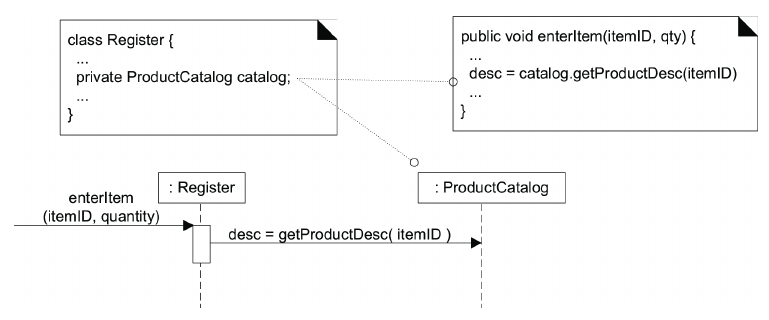
\includegraphics[scale=0.6]{Immagini/Schermata_20260621_223015.png}
\end{figure}

\subsection{Visibilità per parametro}
Avviene quando \uline{l'oggetto B viene passato come parametro all'iterno di un metodo dell'oggetto A}.

Si tratta di una visibilità relativamente \textbf{temporanea}, in quanto è valida ed \uline{esiste esclusivamente per la durata dell'ambito del metodo in cui è stata passata}

\begin{figure}[H]
    \centering
    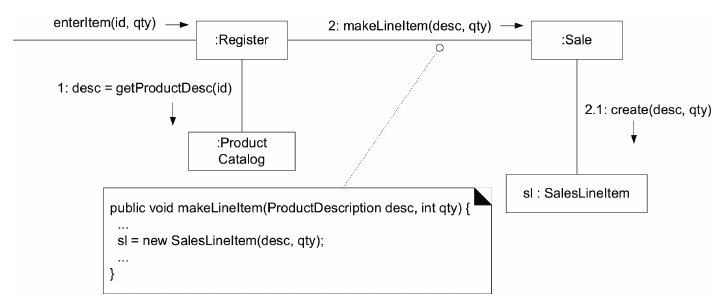
\includegraphics[scale=0.75]{Immagini/Schermata_20260621_223319.png}
\end{figure}

\subsection{Visibilità locale}
Si manifesta quando \uline{l'oggetto B è dichiarato come un oggetto locale all'interno di un metodo di A}.

Anch'essa è una visibilità relativamente \textbf{temporanea} \uline{limitata all'ambito del metodo}.

Può essere ottenuta in 2 modi:
\begin{itemize}
    \item Creando una nuovo istanza locale e assegnandola a una variabile
    \item Assegnando a una variabile locale l'oggetto restituito dalla chiamata a un altro metodo
\end{itemize}

\subsection{Visibilità globale}
Si ottiene quando \uline{l'oggetto B è dichiarato in modo da essere visibile globalmente ad A}.

È una visibilità relativamente \textbf{permanente} e \uline{si realizza assegnando un'istanza a una variabile globale}

\section{Trasformazione della visibilità}
La visibilità \textbf{non è un concetto statico}, ma \uline{le diverse forme di visibilità possono mutare} ed essere convertite l'una nell'altra durante l'esecuzione nel codice.

\subsection{Da visibilità locale a visibilità per parametro}
Si verifica quando un oggetto istanziato o recuperato localmente all'interno di un metodo (visibilità locale) viene passato come argomento (parametro) nella chiamata a un altro metodo.

\subsection{Da visibilità per parametro a visibilità per attributo}
Da visibilità per parametro a visibilità per attributo: È una pratica comune nei metodi di inizializzazione, come i costruttori. 

Un oggetto viene passato in ingresso a un metodo come parametro (visibilità temporanea) e, all'interno di quel metodo, viene assegnato a una variabile di istanza della classe, trasformandosi a tutti gli effetti in un attributo stabile nel tempo.